% !TEX root = ../main.tex
\newpage
\section{\mywork Emerging Network Topologies} \label{sec:EmergingNetworkTopologies}
%\textcolor{red}{TODO}: \textsl{explain in detail how the different methods \cref{eq:KempterSTDPFormulation2,eq:SongSTDPFormulation} will be implemented, using \STDP coupled with \IP.}

We will now investigate what topologies emerge from the learning procedures described in Chapter \ref{sec:HebbianLearningAndSynapticPlasticity}. Are the approaches presented in \cite{Kempter1999, Song2000, Song2017, ChrolCannon2012} plausible within the context of the Theta model? Do we obtain similar results concerning synchronisation and topology? Is there a reason for only allowing the network to make excitatory ($K_{ij} \geq 0$) connections? 

\subsection{Conditions of the network}
As we saw in Chapter \ref{sec:MFRs}, the typical ranges for the coupling strength $\kappa$ and the mean excitability $\eta_0$ to alter the macroscopic state of the network drastically are fairly large. Using the Kempter method \eqref{eq:KempterSTDPFormulation2}, there is no limit on the magnitude of $K$, though initial activity of the node degrees was observed within the interval [-100, 100]. 

When using the Song method \eqref{eq:SongSTDPFormulation} we will constrain $-K^{\rm max} \leq K_{ij} \leq K^{\rm max}$ to allow neurons to both exhibit exitatory and inhibitory behaviour. When testing different values of $K^{\rm max}$ no significant difference was observed in the results, except the time of reaching convergence of $\kmean$. To optimally compare the two methods we will use $K^{\rm max}$ = 100. $K_{ij}$ is initialised using a uniform distribution over $[-K^{\rm max}, K^{\rm max}]$, as to minimise influence of the initial distribution on the resulting topology.\\

The networks we will study consist of 100 Theta neurons, as the computational task of numerically solving the learning equations until convergence is a heavy one. Larger networks are more difficult to simulate, but smaller networks might be more susceptible to the stochastic behaviour of a few neurons. The networks will be initialised with $\theta_i$ equidistantly distributed over $\T$, so that $| Z(0) |$ = 0 exactly. The excitabilities $\eta_i$ are set to zero for all neurons. 
When investigating \STDP + \IP, the excitability is allowed to change over the same domain as $K_{ij}$, in accordance to our comments on $\eta_i$ and $I_i$ cancelling each other out. Therefore we take $\eta_{\max} = K^{\rm max}$ and just like $K_{ij}$, $\eta_i$ is using a uniform distribution over $[-\eta_{\max}, \eta_{\max}]$.


\subsection{Tuning hyperparameters for \texorpdfstring{$W_K$}{TEXT}}
We decided to scale all learning windows presented in Chapter \ref{sec:HebbianLearningAndSynapticPlasticity} to the same order of magnitude, to make for a fair comparison of the learning dynamics over time. What is left now is to tune the hyperparameters $w^{\mathrm{in}}$ and $w^{\mathrm{out}}$. Looking at Figure \ref{fig:KempterWinWout}, we can see that we cannot simply use the same magnitude as the learning window: the dynamics are disturbed by the large discrete changes induced by $w^{\mathrm{in}}$ and $w^{\mathrm{out}}$. A better solution is obtained by using $w^{\mathrm{in}}$ = 10$^{-3}$.

\begin{figure}[H]
\centering
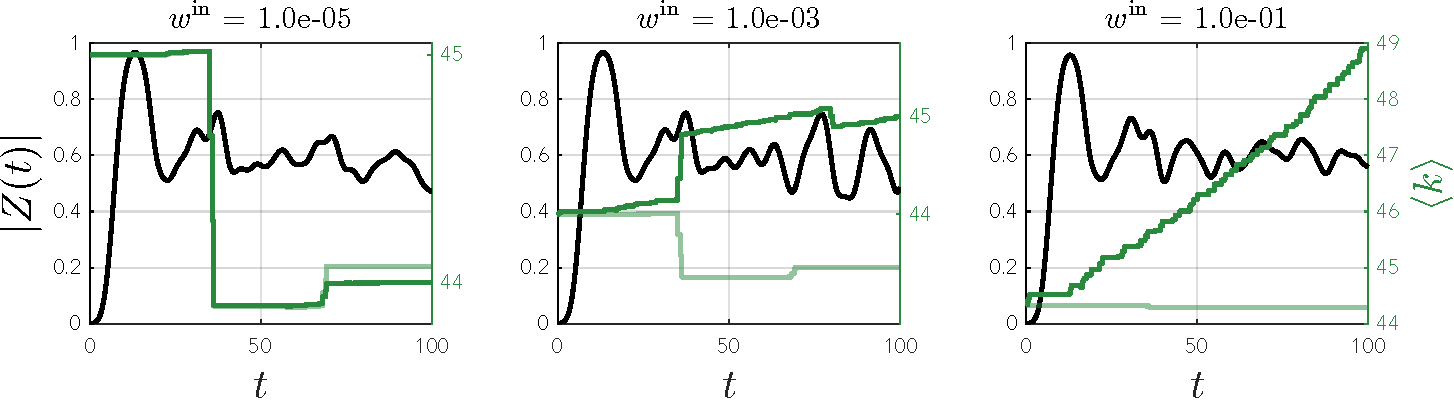
\includegraphics[width = \textwidth]{../Figures/Learning/KempterWinWout.pdf}
\caption{Tuning of the hyperparameters $w^{\mathrm{in}}$ and $w^{\mathrm{out}} = -1.0475  w^{\mathrm{in}}$. The order parameter $Z(t)$ is given in black and the mean network degree $\kmean$ in green. $Z$ is initialised as zero and quickly becomes non-zero. When neurons start bursting we can see a big drop in synchronisation, and a large increase in $\kmean$, meaning that the \STDP method works. Left: the learning dynamics with zero weights, as a benchmark. Middle: the learning dynamics for small, non-zero weights. The mean coupling strength is higher, but the overall synchronisation is lower. This might yield an interesting topological structure. Right: the learning dynamics with the same magnitude as the learning window disturb the learning process.}
\label{fig:KempterWinWout}
\end{figure}


\subsection{Results of \STDP} \label{sec:STDPlearning} %applied to networks of theta neurons 
We can now use the Kempter method and its corresponding learning window and compare it to the Song method and the bi- and triphasic learning windows. The results are shown in Figure \ref{fig:STDP}. It is remarkable how easily the different methods can be recognised, like the influence of the sign and magnitude of the correlation: using $W_C$ yields the most evidence of having adapted. Interestingly, the in- and outdegrees are remarkably similar, and this might endorse our method of obtaining an asymmetrical adjacency matrix by using $\koutb = \permute ( \kinb )$. \\

In the first column of plots, we can see the overall synchronisation of the network and its mean node degree as it learns over time. The Kempter method does not seem to converge for any time period under the circumstances described before. We find the network right before larger node degrees start taking off to higher orders, and remarkably the synchronisation is very low. This might be due to the fact that the modus of $K$ lies close to zero.

The coupling matrix does not seem to contain a lot of structure: a high number of nodes have only a low degree, and so most of the network topology disappears as grey lines. The nodes with very high or very low degrees are sparsely distributed across the matrix. When we look at the histogram underneath, a lognormal shape can be identified. Remember that no constraints are applied to $K$, so its is remarkable a structure seems to appear. Underneath, we can see the node degrees follow a clear correlation, with a more clustered behaviour for high degrees. \\

In the second column we can see the results of using the Song method with $W_S$. The learning behaviour is more regular and we can observe that with an increasing network connectivity we obtain increased synchronisation. Convergence is near completion, and we can see the separation between two clusters of node degrees in the high-contrast image of $K$, and in all histograms and plots. We can interpret the scatterplot of $\kin$ versus $\kout$ as a small group of nodes of varying degrees, and a large group of node degrees at the limits, as the definition of the degree vectors \eqref{eq:redefineFromK} takes only the absolute value. Most neurons see their synaptic strength decreased by the negative correlation. There is only a small fraction of oscillators that has learned to spike at the right time and manages to keep increasing its synaptic strength and eventually ends up at $K^{\rm max}$. \\%The dichotomy may also be found in the shape of the learning window: the large difference

In the third column we can see the results of using the Song method with $W_C$. Convergence to a steady-state happens much more steadily, and also the synchronisation benefits from this approach. The coupling matrix shows an even stronger partition, as even fewer neurons manage to learn to spike at the right interval. It is even more clear here how well the network is split into two distinct groups with either high or low node degrees.\\

It is useful to review our choice to define $\kin$ from the absolute value of $K_{ij}$. One can see this operation as folding the histogram of $K$ in half at 0, and one can argue that inherently information is lost. However, when not accounting for the sign of the synaptic strength, they might cancel out and a node degree of zero might be found for even the best connected neurons. What we do lose is the ability to see positive or negative correlation, but that information can be found from the learning window, or from the mean value of the histogram of $K$.


\subsection{Results of \STDP + \IP} \label{sec:STDPandIPlearning}
When introducing intrinsic plasticity, the expected changes to $\eta_i$ counteract $K$ as expected: $\eta_i$ is cranked up to the largest possible value for virtually all neurons, but it seems to have an effect on the topology. The results are shown in Figure \ref{fig:STDPandIP}. 

We find the Kempter method again on the verge of exploding, where nodes with a large degree (both negative and positive) are about to take off to even larger orders of magnitude. The overall structure is similar as before, but the positive correlation between in- and out-degrees is stronger. The synchronisation is again remarkably low, as the modus of $K$ lies close to zero again. It seems like $K$ is more symmetric than before.

The Song method benefits from a faster convergence, which we can see in the second and third column. This is likely due to the neurons becoming less susceptible with an increased excitability. A more uniform distribution of node degrees can be found between the two extrema, as convergence has halted. For both methods the dichotomy between low and high degree nodes is more clear, especially for $W_C$.

\subsection{Interpretation of the results}
When comparing the results of \STDP with and without \IP, we can observe that including the excitability as a learnable parameter, the learning process is more stable, and convergence can be achieved using the Song method. A relation appears to exist between the in- and out-degrees of different nodes, and the degree distributions appear even more similar.

It is remarkable that in only few cases the network of Theta neurons finds an equilibrium state. These can be recognised immediately, as all learning stops and the synchronisation is 1. It appears that the changing network topology is enough to sustain a globally periodic spiking regime, though we assume individual neurons switch between the excitable and bifurcation regimes as well, due to the highly variable nature of the term $\eta_i + I_i$, which is right at the heart of our learning. \\

As speculated before, we can also interpret the convergence of the results as $\eta_i$ and $K_{ij}$ cancelling each other out. Learning only occurs when the neurons are spiking, and as this is regulated by $W$ we want the firing rates to be close to the maximum of the learning window. That would result in the largest desirable increase in $K$, and therefore a large incoming current $I_i$. As $N$ = 100, we can easily expect $I_i$ to be around that number. With \IP however, when $\eta_i + I_i$ is close to zero, the time required to spike can be very long, as we saw in Chapter \ref{TheThetaNeuronModel}. Only nodes with the highest coupling strength are able to overcome this threshold.

\newpage
\begin{figure}[H]
\centering
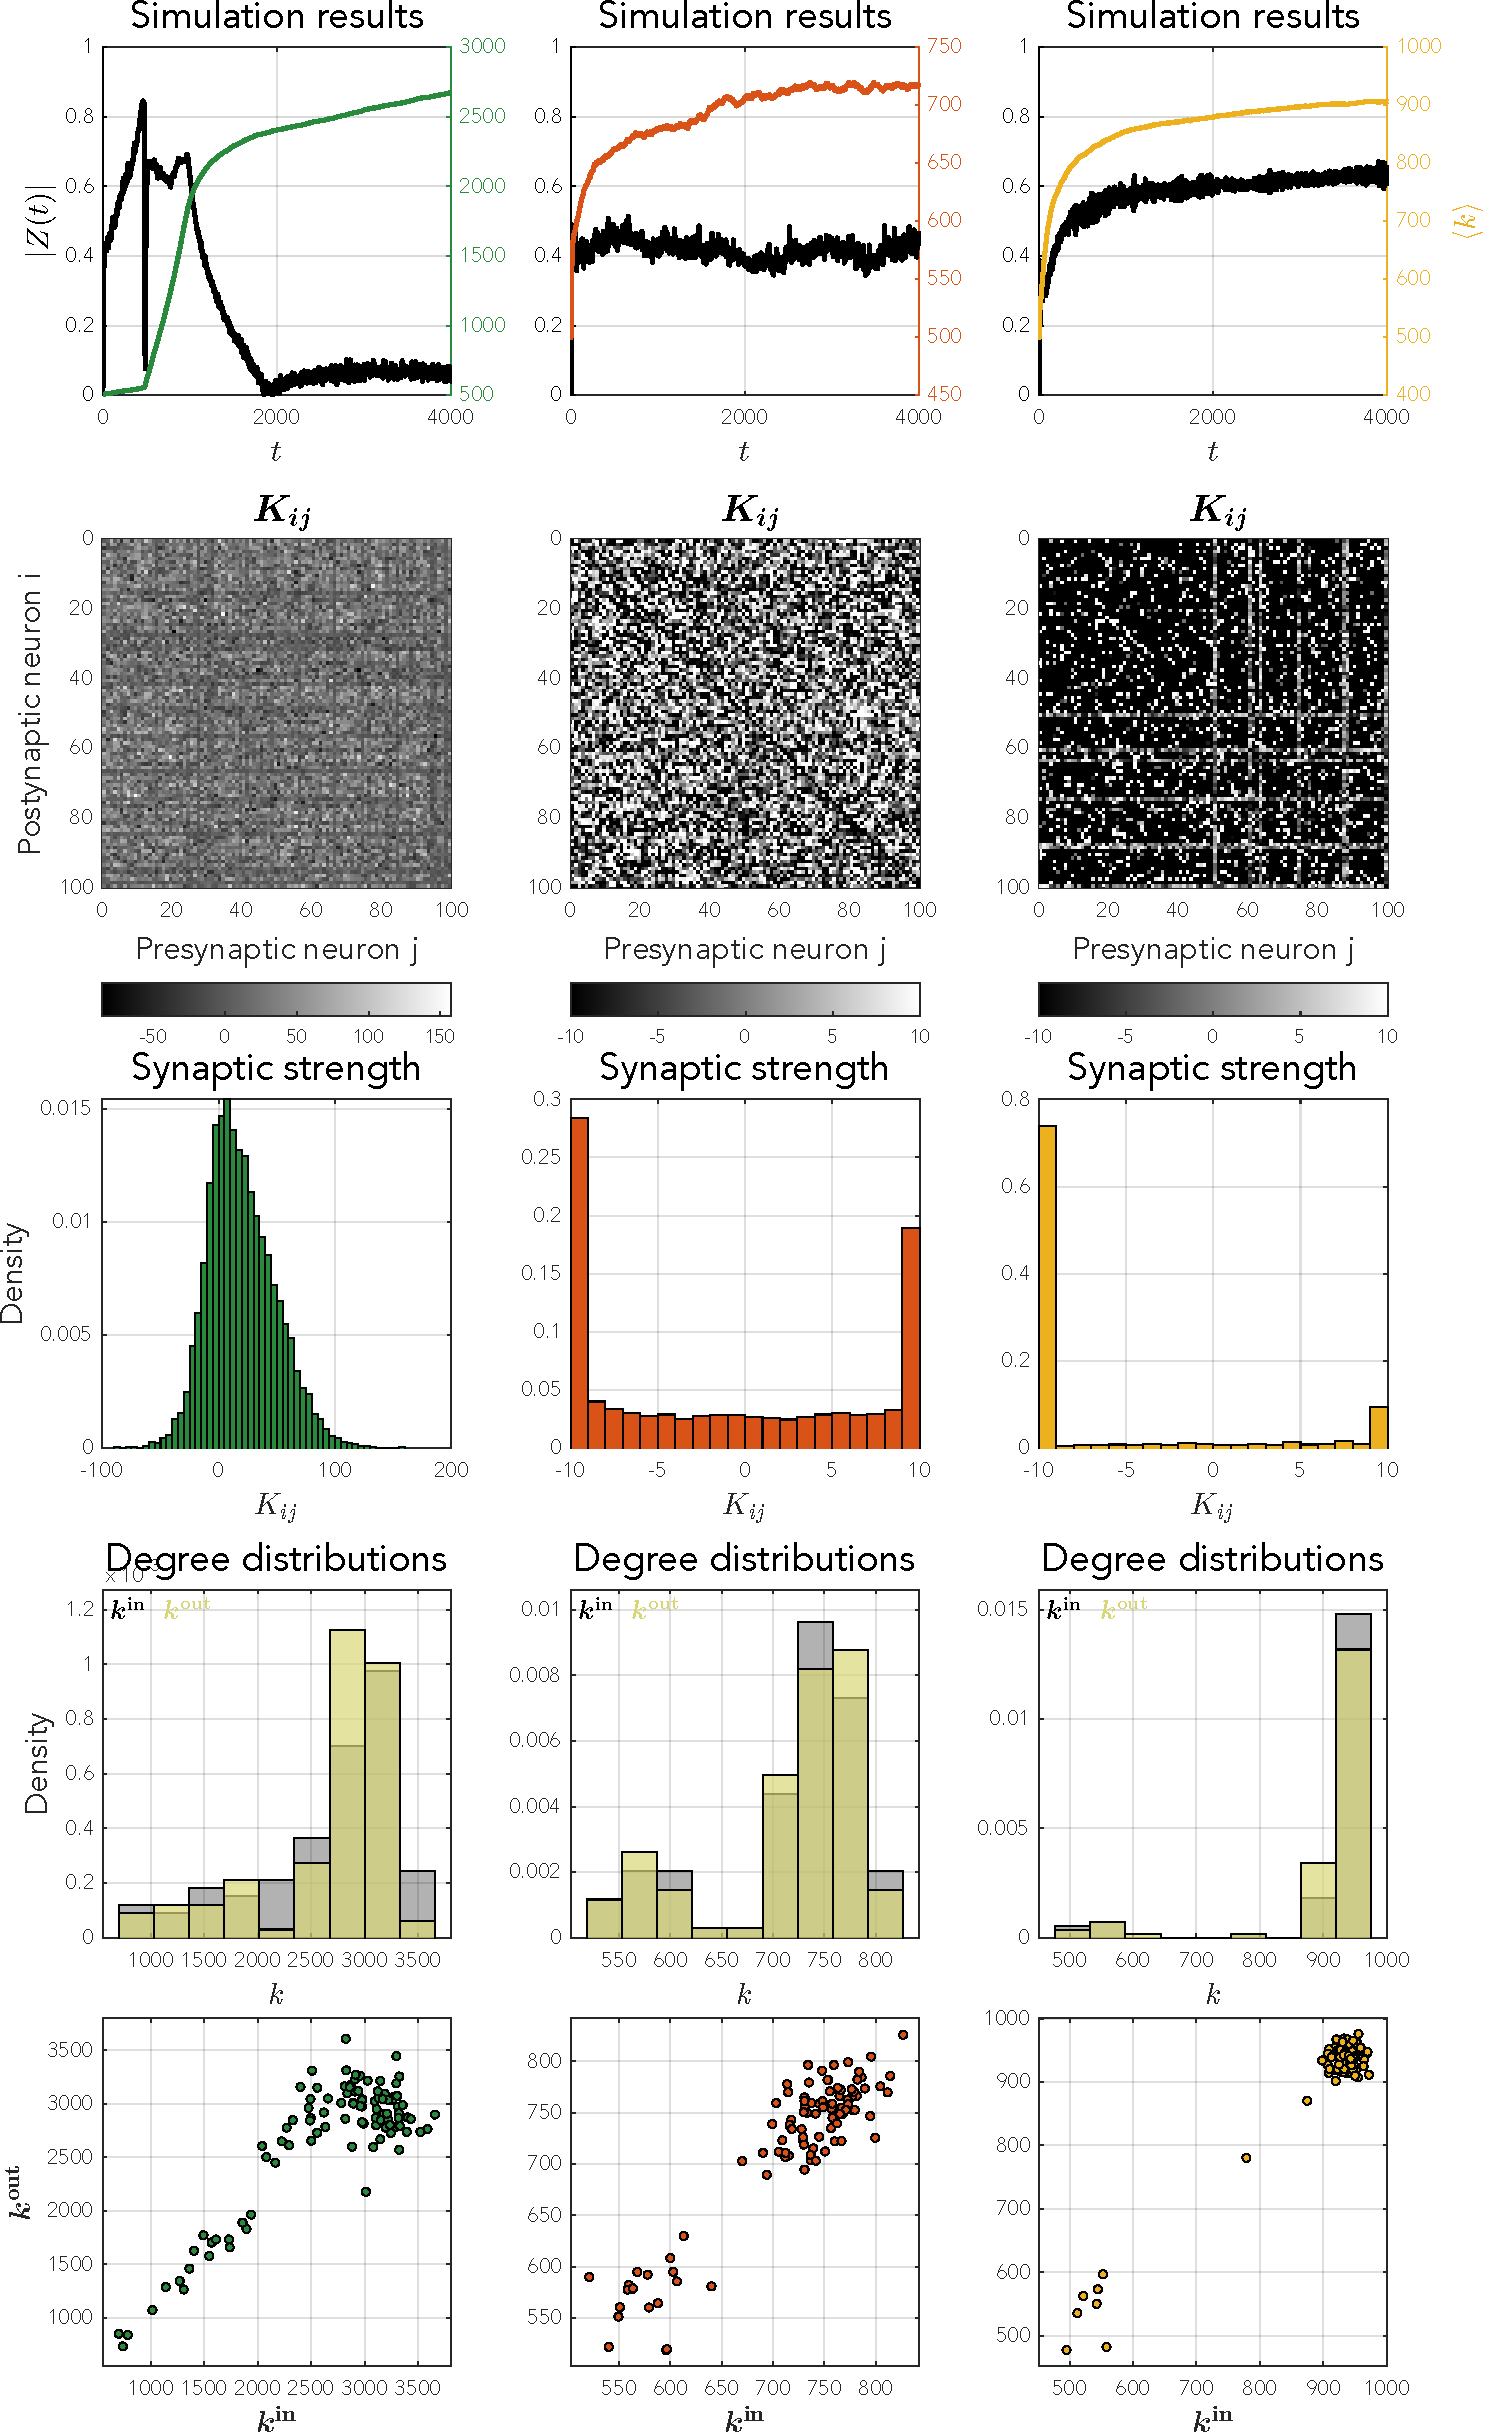
\includegraphics[height = \textheight]{../Figures/Learning/STDP.pdf}
\caption{Results of the \STDP learning.}
\label{fig:STDP}
\end{figure}

\begin{figure}[H]
\centering
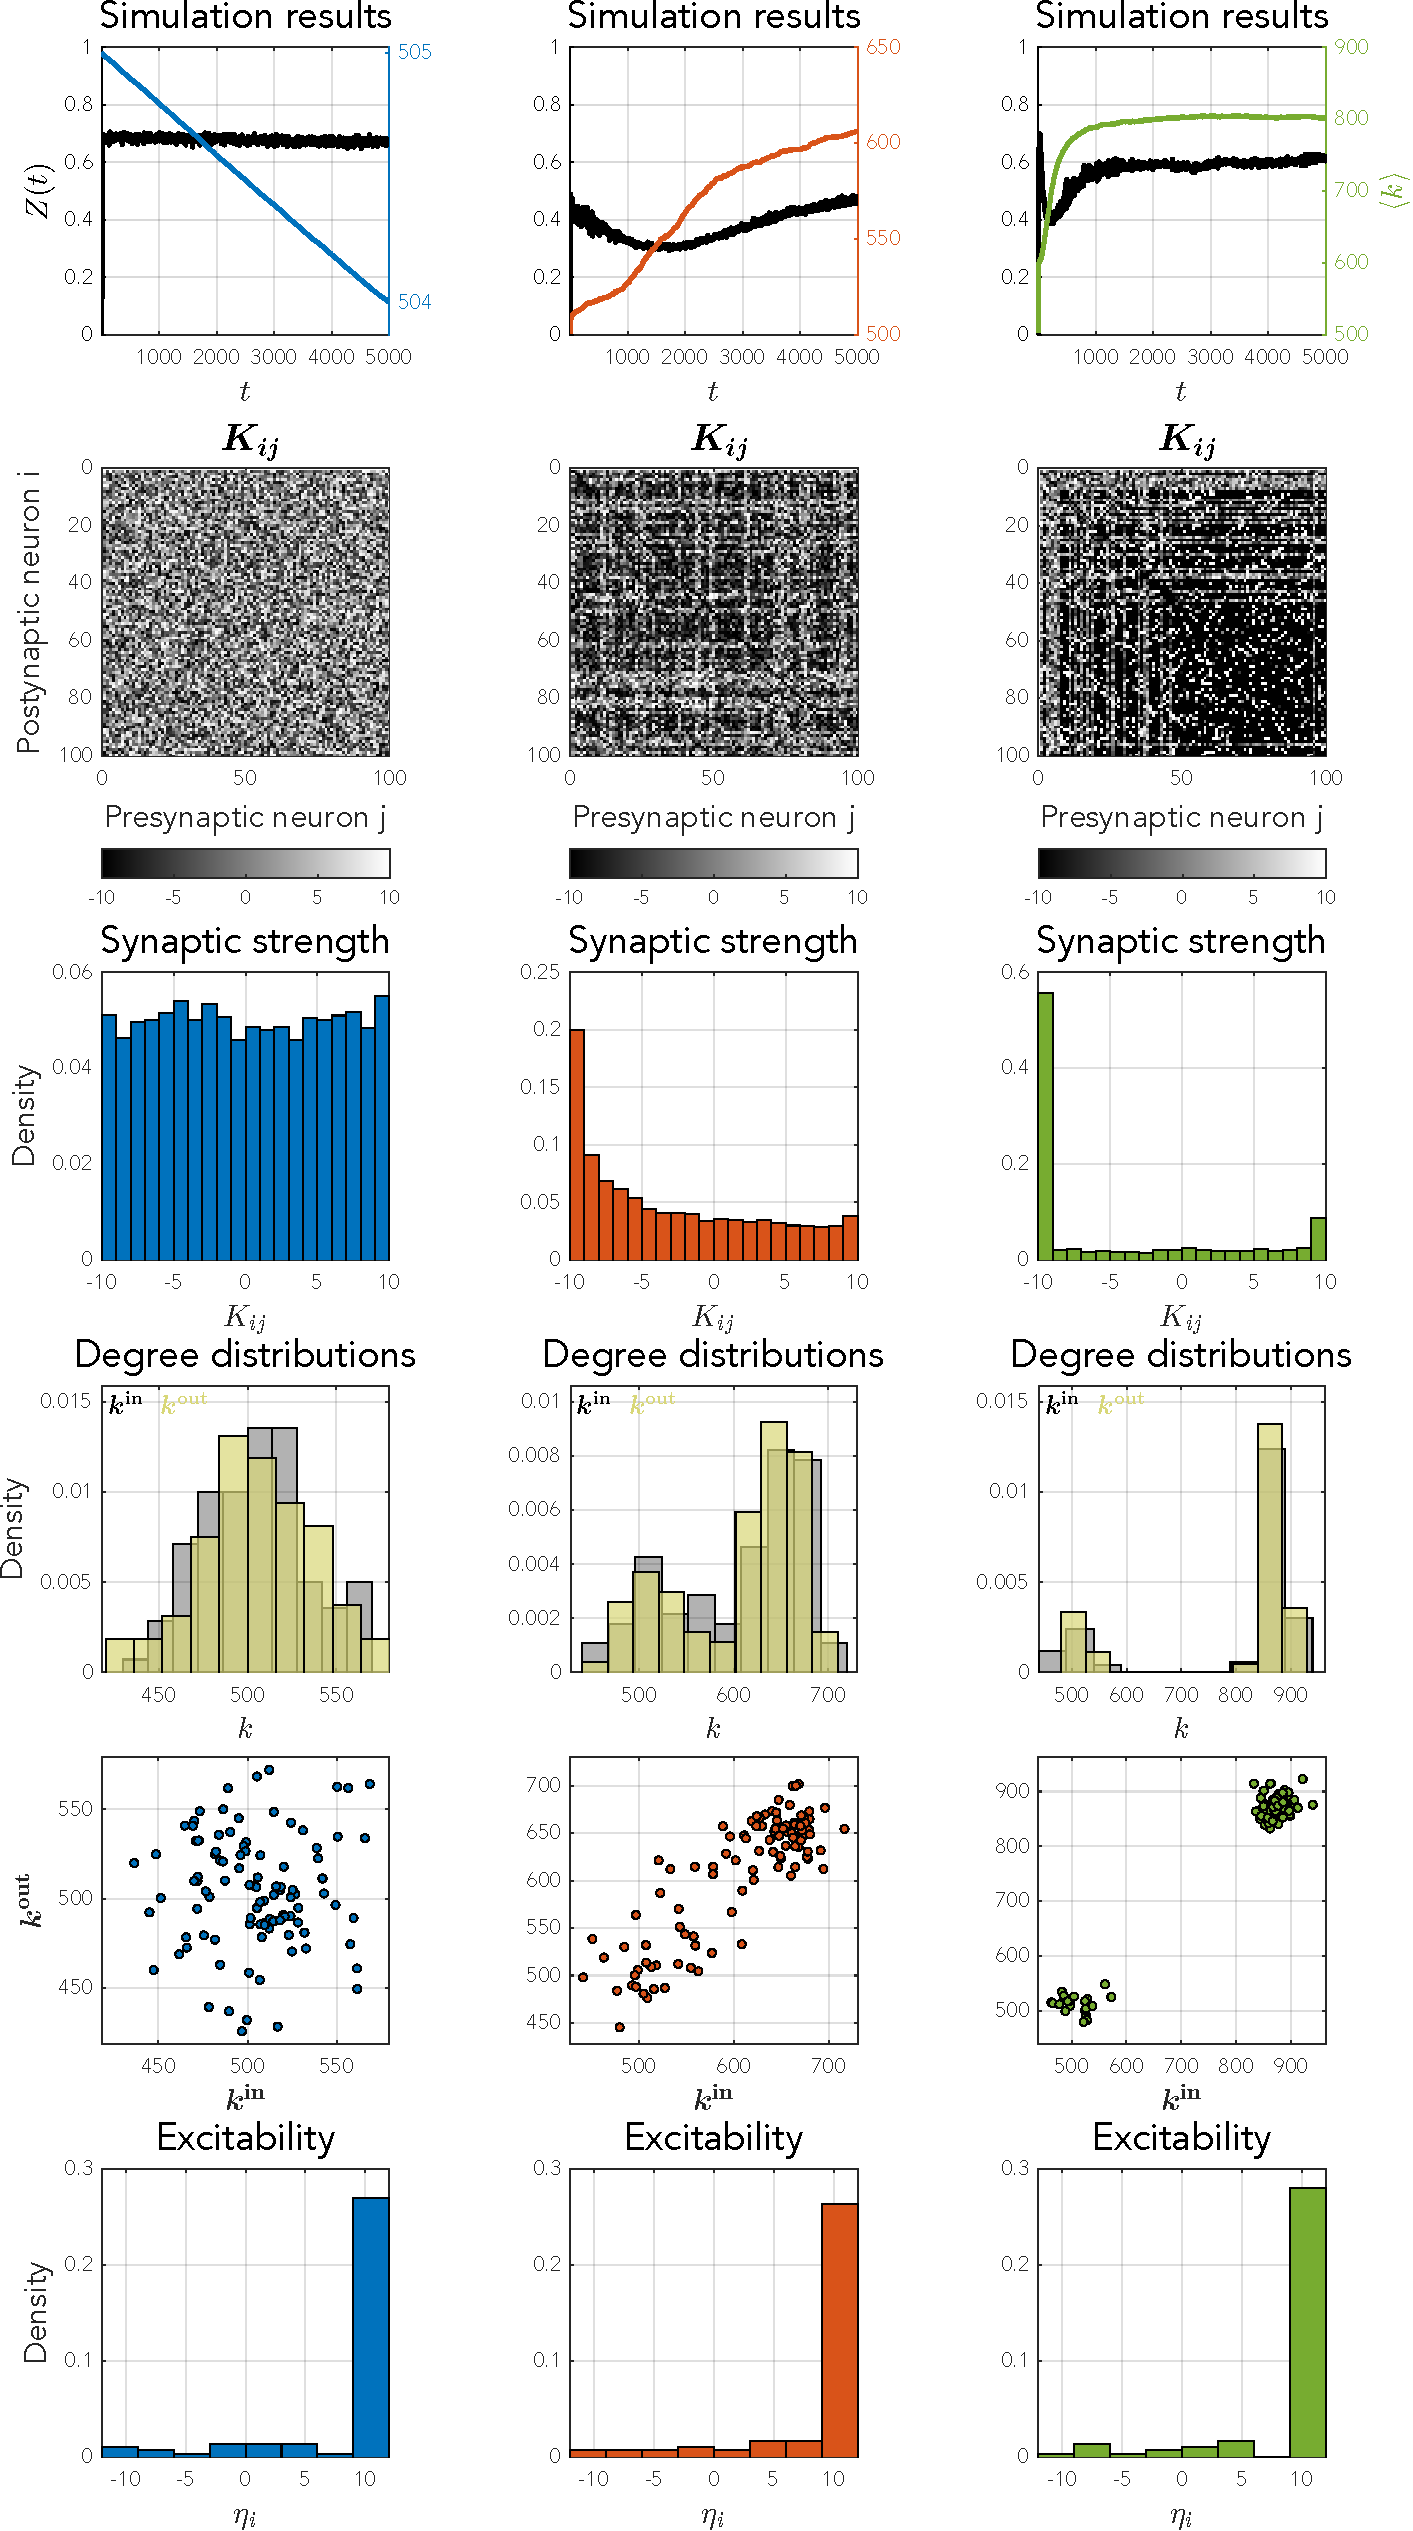
\includegraphics[height = \textheight]{../Figures/Learning/STDPandIP.pdf}
\caption{Results of the \STDP learning with \IP learning.}
\label{fig:STDPandIP}
\end{figure}

